\section{Experiment Results}
\label{experiment}
In this section, we evaluate the method of random walk with restart on the combined RDF bipartite graph for discovering semantic associations. We conducted a series of experiments to highlight the effect of the incorporating the ontologies in the mining task. First, we evaluated our methods on a commonly used \emph{shopping cart} dataset together with a manually created ontology describing the subsumption hierarchy for grocery items.  Then, we applied our method to actual \emph{electronic health records} to highlight its scalability and applicability to the biomedical domain. The sizes of the datasets used in our experiments in terms of numbers of RDF triples are summarized in Table~\ref{tbl:exp_overview}.


\begin{table*}[tbh]\scriptsize
\begin{center}
\begin{tabular}{c|c|c|c}
\hline
    & \# data triples & \# \emph{is\_a} relationships & \# other relationships \\
    \hline
  Shopping cart     &  8,481       & 127       &    0\\
  Healthcare &  10,000,257  & 1,048,604 &    43,780\\
  \hline
\end{tabular}
\end{center}
\caption{\label{tbl:exp_overview} The \emph{shopping cart} and \emph{healthcare} datasets vary in size of data, size of ontology, and in the kinds of relationships defined by the ontology.}
\end{table*}

%
%\subsection{Shopping Cart Dataset}
%\subsubsection{Data}
%The shopping cart dataset contains purchase information on 100 grocery items for 2,127 shopping orders. The data tuples can be represented as 8,481 RDF statements.  We introduce a small ontology to organize the grocery items into a subsumption hierarchy (see Figure~\ref{fig:foodmart_onto} for example) with 28 internal nodes.  Since the 100 grocery items are mostly at the leaf level, this results in a total of 127 new RDF statements to incorporate the ontology with the data.
%
\begin{figure*}[tbh]
\begin{center}
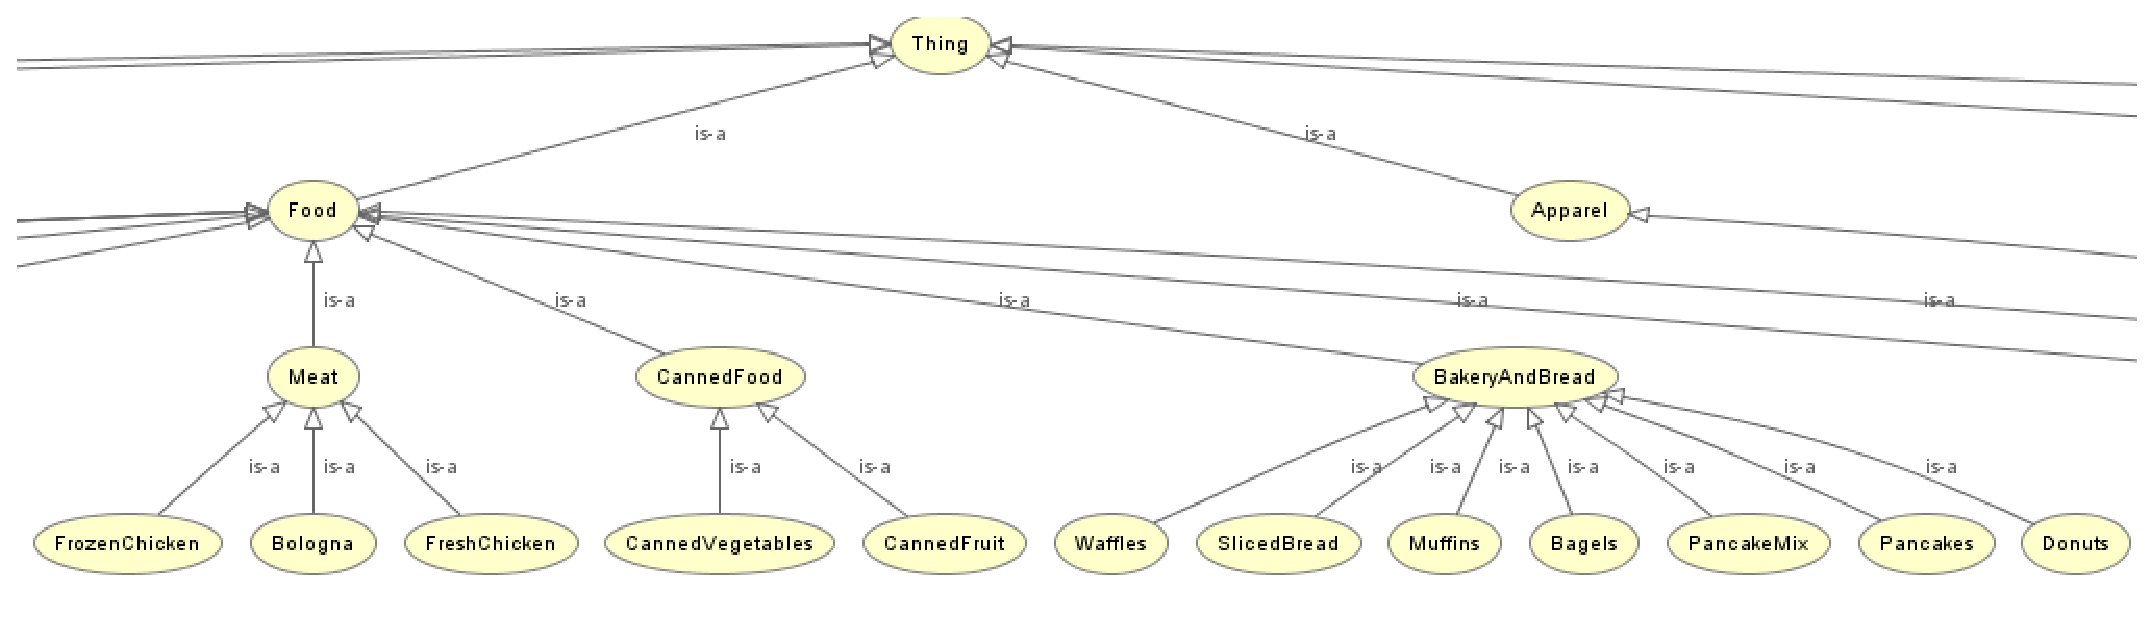
\includegraphics[width=.9\textwidth]{fig/foodmart_onto2.eps}
\end{center}
\caption{\label{fig:foodmart_onto} A portion of the manually created shopping cart ontology.}
\end{figure*}
%
%\subsubsection{Results}
%Items associated with the query term ``toothbrush'' are ranked by the strength of semantic association in Table~\ref{tbl:foodmart_comp}.
%When the ontology is ignored (Table~\ref{tbl:foodmart_comp} (A)), associated items are either hub nodes (with many edges linking to other items) or frequently co-occur with the query item, as in traditional association rule mining over transactional data. Conversely, using only the ontology graph (Table~\ref{tbl:foodmart_comp} (B)) returns the neighborhood of terms in the rdfs:subClassOf lattice. Combining both the ontology and data (Table~\ref{tbl:foodmart_comp} (C--E)),  yields a variety of mixtures of these associations. In a rough sense, it conforms to the ratio of the size of ontology graph and data graph as well (see Table~\ref{tbl:exp_overview}).
%\begin{table*}[tbh]\scriptsize
%\begin{center}
%\begin{tabular}{ c c || c c || c c || c c }
%\hline
%\multicolumn{2}{c||}{$w_o=0$, $w_d=1$}&\multicolumn{2}{c||}{$w_o=1$, $w_d=0$}&\multicolumn{2}{c||}{$w_o=1$, $w_d=1$}&\multicolumn{2}{c}{$w_o=10$, $w_d=1$}    \\
%\hline
%item	&	p(\%)	&	item	&	p(\%)	&	item	&	p(\%)	&	item	&	p(\%)	\\
%\hline															
%Soup	&	0.42	&	PersonalHygiene	&	12.55	&	PersonalHygiene	&	0.74	&	PersonalHygiene	&	3.97	\\
%Cookies	&	0.41	&	Snack	&	0.86	&	Soup	&	0.41	&	NasalSprays	&	0.41	\\
%NasalSprays	&	0.38	&	Health	&	0.64	&	Cookies	&	0.4	&	Soup	&	0.34	\\
%Popcorn	&	0.32	&	Sponges	&	0.57	&	NasalSprays	&	0.37	&	Cookies	&	0.34	\\
%PaperWipes	&	0.29	&	Soap	&	0.57	&	Popcorn	&	0.31	&	Mouthwash	&	0.3	\\
%FrozenVegetables	&	0.29	&	Shampoo	&	0.57	&	FrozenVegetables	&	0.29	&	Popcorn	&	0.25	 \\
%PersonalHygiene	&	0.26	&	NasalSprays	&	0.57	&	PaperWipes	&	0.28	&	FrozenVegetables	&	0.24	 \\
%DriedFruit	&	0.25	&	Mouthwash	&	0.57	&	DriedFruit	&	0.25	&	PaperWipes	&	0.23	 \\
%Milk	&	0.25	&	Conditioner	&	0.57	&	Milk	&	0.25	&	DriedFruit	&	0.22	\\
%Mouthwash	&	0.24	&	MealCourse	&	0.54	&	Mouthwash	&	0.23	&	Milk	&	0.21	\\
%\hline
%\multicolumn{2}{c}{(A)}  &   \multicolumn{2}{c}{(B)}  &   \multicolumn{2}{c}{(C)}  &   \multicolumn{2}{c}{(D)}  \\
%\end{tabular}
%\end{center}
%\caption{\label{tbl:foodmart_comp} Foodmart items ranked by the strength of semantic association to the query term ``toothbrush.'' The ranking, $p(\%)$, denotes the steady-state probability.}
%\end{table*}
%
%Because we created the ontology to illustrate our point, we filter out all terms exclusive to the ontology in Table~\ref{tbl:foodmart_comp2} to elicit top items associated with the query term ``soup."   The pair \emph{``soup"-``cold remedies"}) (ranked 34th with data graph, not shown in the table) is one that we can find, which makes sense but never co-occurs in the data alone and would not be picked up by traditional methods.
%
%%Finally we tested our methods on the dataset of electronic health records of real patients. This dataset is different from the above two datasets not only in scale but also in practical importance as described in the following.
%% state in very clear sentence what the conclusion is, what is the take-home message you want them to see? xxx
%
%% why is this interesting? what should we have learned? xxx
%
%%finally, lead-in to final experiment... we finally did this last experiment because:  1) its huge, 2) its important to people to solve xxx
%
%\begin{table*}[tbh]\scriptsize
%\begin{center}
%\begin{tabular}{ l r | l r || l r | l r }
%\hline
%\multicolumn{4}{c||}{$w_o=0$, $w_d=1$}  &   \multicolumn{4}{c}{$w_o=1$, $w_d=0$}\\
%\hline
%item	&	p(\%)	&	item	&	p(\%)	&	item	&	p(\%)	&	item	&	p(\%)	\\
%\hline
%Cheese	&	0.38	&	Preserves	&	0.19	&	TVDinner	&	0.46	&	Sponges	&	0.06	\\
%Cookies	&	0.32	&	Juice	&	0.17	&	Pizza	&	0.46	&	Soap	&	0.06	\\
%DriedFruit	&	0.32	&	Lightbulbs	&	0.17	&	Pasta	&	0.46	&	Shampoo	&	0.06	\\
%Wine	&	0.24	&	PaperWipes	&	0.16	&	HotDogs	&	0.46	&	NasalSprays	&	0.06	\\
%CannedVegetables	&	0.23	&	Pizza	&	0.16	&	Hamburger	&	0.46	&	Mouthwash	&	0.06	\\
%FrozenVegetables	&	0.23	&	Nuts	&	0.16	&	FrenchFries	&	0.46	&	Conditioner	&	0.06	\\
%Cereal	&	0.22	&	Popcorn	&	0.16	&	DeliSalads	&	0.46	&	Ibuprofen	&	0.06	\\
%Milk	&	0.22	&	Chips	&	0.16	&	DeliMeats	&	0.46	&	ColdRemedies	&	0.06	\\
%ChocolateCandy	&	0.19	&	Eggs	&	0.16	&	Sunglasses	&	0.07	&	Aspirin	&	0.06	\\
%Waffles	&	0.19	&	TVDinner	&	0.15	&	Toothbrushes	&	0.06	&	Acetominifen	&	0.06	\\					 
%\hline
%\end{tabular}
%\end{center}
%\caption{\label{tbl:foodmart_comp2} Foodmart items ranked by the strength of semantic association to the query term ``soup.'' The ranking, $p(\%)$, denotes the steady-state probability. Terms exclusive to the Foodmart ontology are filtered out.}
%\end{table*}


\subsection{Shopping Cart}
\subsubsection{Dataset}
The shopping cart dataset contains purchase information on 100 grocery items (represented by boolean column headers) for 2,127 shopping orders (corresponding to tuples) from a Foodmart. We first construct an RDF bipartite graph from the dataset by transforming the table to 8481 RDF statements.

Besides, we manually create an ontology to organize the grocery items into a subsumption hierarchy (see Figure~\ref{fig:foodmart_onto} for example). In this process, we introduce 28 parent nodes (the 100 grocery items appeared in the data are mostly at the leaf level) from which derive a total of 127 RDF statements. As the size of this dataset is fairly small, the calculation of similarity ranking for a given term is fast. In the following we highlight the effect of incorporation of ontology by comparing results obtained with and without ontologies.


\subsubsection{Results}
In Table~\ref{tbl:foodmart_comp}, results of items ranked by the strength of semantic association with regard to a query term ``Toothbrush" under various combinations of parameters are demonstrated side-by-side for comparison. We first show the result ranked by co-frequency in Table~\ref{tbl:foodmart_comp}(A) as a baseline. Then, we observe that without using ontology, performing random walk with restart on the data graph (Table~\ref{tbl:foodmart_comp}(A)) starting from ``toothbrush" yields similar results to the work reported in~\cite{LiuEtal11} based on random walk commute time similarity. Items ranked high in this setting where only the data graph is considered are typically either hub nodes (with many edges linking to other items) or co-frequent with the query item (many edges connecting them). Second, applying the same similarity ranking method solely on the ontology graph (Table~\ref{tbl:foodmart_comp}(C)) gives a list of association based on the graph-configuration of the ontological structure (in this case, the rdfs:subClassOf lattice). The items that are considered most similar to the query term ``Toothbrush" is its immediate parent class ``PersonalHygiene," followed by some most derived classes at the same level of ``PersonalHygiene" and then siblings of ``Toothbrush" itself. Next, Table~\ref{tbl:foodmart_comp}(D)--(F) demonstrate the results of mining on the combined graph with different ratios of weights assigned to ontology edges and data edges respectively. It is obvious that these results can be seen as a mix of the data-only and ontology-only results with various emphasis on the data or ontology. We can observe that when $w_o/w_d=20$ the ontology and data appear to have equal significance in determining the ranking ($w_o$ is the weight of ontology edges (i.e., rdfs:subClassOf) and $w_d$ is the weight of data edges). In a rough sense, it conforms to the ratio of the size of ontology graph and data graph as well (see Table~\ref{tbl:exp_overview}). In reality, the appropriate ratio for the edge weights is not only dependent on the size of graphs but also the specific configuration of the graph (depth, average degree, etc). Moreover, specifying the ratio of prior knowledge in ontologies and inductive evidences in data that one wants to employ for discovering new patterns is a highly empirical process. Multiple pilot trials may need to be carried out for the optimal ratio before it is applied to the real application.

\begin{table*}[tbh]\scriptsize
\begin{center}
\begin{tabular}{ c c || c c | c c }
\hline
\multicolumn{2}{c||}{ranked by co-frequency}&\multicolumn{2}{c|}{w/ data only}&\multicolumn{2}{c}{w/ ontology only}\\
\hline
item	&	freq	&	item	&	p(\%)	&	item	&	p(\%)	\\
\hline											
PaperWipes	&	8	&	Soup	&	0.42	&	PersonalHygiene	&	12.55	\\
Popcorn	&	7	&	Cookies	&	0.41	&	Snack	&	0.86	\\
Soup	&	6	&	NasalSprays	&	0.38	&	Health	&	0.64	\\
NasalSprays	&	6	&	Popcorn	&	0.32	&	Sponges	&	0.57	\\
Cookies	&	6	&	PaperWipes	&	0.29	&	Soap	&	0.57	\\
Spices	&	5	&	FrozenVegetables	&	0.29	&	Shampoo	&	0.57	\\
Soda	&	4	&	PersonalHygiene	&	0.26	&	NasalSprays	&	0.57	\\
Shrimp	&	4	&	DriedFruit	&	0.25	&	Mouthwash	&	0.57	\\
FlavoredDrinks	&	4	&	Milk	&	0.25	&	Conditioner	&	0.57	\\
Dips	&	4	&	Mouthwash	&	0.24	&	MealCourse	&	0.54	\\
\hline
\multicolumn{6}{c}{~}\\
\multicolumn{2}{c}{(A)}  &   \multicolumn{2}{c}{(B)}  &   \multicolumn{2}{c}{(C)}  \\
\multicolumn{6}{c}{~}\\
\end{tabular}

\begin{tabular}{ c c | c c | c c }
\hline
\multicolumn{2}{c|}{$w_o=1$, $w_d=1$}&\multicolumn{2}{c|}{$w_o=10$, $w_d=1$}&\multicolumn{2}{c}{$o_w=20$, $o_d=1$}\\
\hline
item	&	p(\%)	&	item	&	p(\%)	&	item	&	p(\%)	\\
				\hline							
PersonalHygiene	&	0.74	&	PersonalHygiene	&	3.97	&	PersonalHygiene	&	6.27	\\
Soup	&	0.41	&	NasalSprays	&	0.41	&	NasalSprays	&	0.5	\\
Cookies	&	0.4	&	Soup	&	0.34	&	Mouthwash	&	0.41	\\
NasalSprays	&	0.37	&	Cookies	&	0.34	&	Shampoo	&	0.31	\\
Popcorn	&	0.31	&	Mouthwash	&	0.3	&	Soup	&	0.29	\\
FrozenVegetables	&	0.29	&	Popcorn	&	0.25	&	Cookies	&	0.29	\\
PaperWipes	&	0.28	&	FrozenVegetables	&	0.24	&	Sponges	&	0.28	\\
DriedFruit	&	0.25	&	PaperWipes	&	0.23	&	Health	&	0.27	\\
Milk	&	0.25	&	DriedFruit	&	0.22	&	Conditioner	&	0.27	\\
Mouthwash	&	0.23	&	Milk	&	0.21	&	Soap	&	0.25	\\
\hline
\multicolumn{4}{c}{~}\\
\multicolumn{2}{c}{(D)}  &  \multicolumn{2}{c}{(E)}  & \multicolumn{2}{c}{(F)}\\
\end{tabular}
\end{center}
\caption[Top results on the Foodmart dataset]{\label{tbl:foodmart_comp} Foodmart items ranked by the strength of semantic association  (i.e., $p(\%)$, the steady-state probability), given the query term ``Tooth Brush."}
\end{table*}

We notice that without any filtering on the ranked semantic associations from the combined graph, the list includes items that never appear in the transactional data. This is because typically the semantic annotation process links table attributes to their most specific matching concept in the ontology which are close to the leaf level. The incorporation of ontology is to aid the mining process, therefore including in the result those parent nodes (e.g.,, ``PersonalHygiene") that never appear in the data is counterintuitive. To overcome this, we can simply filter out those items exclusive to the ontology. Table~\ref{tbl:foodmart_comp2} shows an example of filtered result given a query term ``soup." The co-frequency of items are also listed for comparison.

%Finally we tested our methods on the dataset of electronic health records of real patients. This dataset is different from the above two datasets not only in scale but also in practical importance as described in the following.
% state in very clear sentence what the conclusion is, what is the take-home message you want them to see? xxx

% why is this interesting? what should we have learned? xxx

%finally, lead-in to final experiment... we finally did this last experiment because:  1) its huge, 2) its important to people to solve xxx

\begin{table*}[tbh]\scriptsize
\begin{center}
\begin{tabular}{ c c c | c c c |}
\hline											
\multicolumn{6}{c|}{w/ data only}\\											
\hline											
item	&	p(\%)	&	freq	&	item	&	p(\%)	&	freq	 \\
\hline											
Cheese	&	0.38	&	98	&	Preserves	&	0.19	&	65	 \\
Cookies	&	0.32	&	96	&	Juice	&	0.17	&	47	\\
DriedFruit	&	0.32	&	87	&	Lightbulbs	&	0.17	&	47	 \\
Wine	&	0.24	&	63	&	PaperWipes	&	0.16	&	55	 \\
CannedVegetables	&	0.23	&	67	&	Pizza	&	0.16	&	46	 \\
FrozenVegetables	&	0.23	&	79	&	Nuts	&	0.16	&	60	 \\
Cereal	&	0.22	&	56	&	Popcorn	&	0.16	&	39	 \\
Milk	&	0.22	&	53	&	Chips	&	0.16	&	46	 \\
ChocolateCandy	&	0.19	&	16	&	Eggs	&	0.16	&	51	 \\
Waffles	&	0.19	&	51	&	TVDinner	&	0.15	&	40	 \\
\hline									
\end{tabular}
\begin{tabular}{ | c c c | c c c }
\hline									
\multicolumn{6}{|c}{w/ onto only}\\											
\hline
item	&	p(\%)	&	freq	&	item	&	freq	&	 p(\%)	 \\
\hline
TVDinner	&	0.46	&	40	&	Sponges	&	21	&	0.06	 \\
Pizza	&	0.46	&	46	&	Soap	&	0	&	0.06	\\
Pasta	&	0.46	&	29	&	Shampoo	&	34	&	0.06	 \\
HotDogs	&	0.46	&	30	&	NasalSprays	&	21	&	0.06	 \\
Hamburger	&	0.46	&	19	&	Mouthwash	&	28	 &	0.06	 \\
FrenchFries	&	0.46	&	37	&	Conditioner	&	12	 &	0.06	 \\
DeliSalads	&	0.46	&	31	&	Ibuprofen	&	18	&	0.06	 \\
DeliMeats	&	0.46	&	37	&	ColdRemedies	&	33	&	0.06	 \\
Sunglasses	&	0.07	&	12	&	Aspirin	&	22	&	0.06	 \\
Toothbrushes	&	0.06	&	13	&	Acetominifen	&	12	 &	0.06	 \\
\hline
\end{tabular}
\end{center}
\caption[Top results on the Foodmart dataset excluding concepts only in\protect\newline the ontology]{\label{tbl:foodmart_comp2} Semantically associated items  for the query term ``Soup," by filtering out those items exclusive to the Foodmart ontology.}
\end{table*}


\subsection{Electronic Health Records}
\subsubsection{Dataset}
In our second evaluation, we analyzed the electronic health records of real patients. The patient clinical note data are from Stanford Hospital's Clinical Data Warehouse (STRIDE). These records archive over 17-years worth of patient data comprising of 1.6 million patients, 15 million encounters, 25 million coded ICD9 diagnoses, and a combination of pathology, radiology, and transcription reports totaling over 9 million clinical notes (i.e., unstructured text).
We obtained the set of drugs and diseases for each patient's clinical note by using a new tool, the \emph{Annotator Workflow}, developed at the National Center for Biomedical Ontology (NCBO), which annotates clinical text from electronic health record systems and extracts disease and drug mentions from the electronic health records.

%In addition to having obvious data-mining applications, the workflow has been used by biomedical researchers to build semantic-search applications, such as the NCBO Resource Index~\cite{jonquet11}, which won the Semantic Web Challenge\footnote{\url{http://challenge.semanticweb.org/}} in 2010. The annotation process utilizes the vast NCBO BioPortal ontology library~\cite{bioportal} to extract information by using a lexicon of over one million terms generated from the relevant ontologies, such as SNOMED-CT, RxNORM, and MedDRA. Furthermore, it also incorporates negation detection --- the ability to discern whether a term is negated with the context of the narrative (e.g., lack of valvular dysfunction). Finally, it uses mappings between terms across ontologies~\cite{ghazvinian09}, which forms a rich knowledge graph %(Figure~\ref{fig:collapse})
%or mega-thesaurus, to normalize the lexicon by reducing the feature set from over one million to merely 11,107 unique drugs and 3,594 unique diseases.

From this set of 1.6 million patients with annotated records, we vectorize texts and turned them into a huge bag-of-word representation, from which an RDF bipartite graph is constructed (including 148 million RDF statements, see Table~\ref{tbl:exp_overview}). we applied our algorithms to all previous records in the patient's timeline, looking at just the set of drugs and their semantically related diseases.  Therefore, at a very simplistic level, the experiment result shows that strong semantically associated items in this context could possibly represent sets of drugs that could lead toward certain diseases.

One strength of the Annotator is the highly comprehensive and interlinked lexicon that it uses. It can incorporate the entire NCBO BioPortal ontology library of over 250 ontologies to identify biomedical concepts from text using a dictionary of terms generated from those ontologies. Terms from these ontologies are linked together via mappings. For this study, we specifically configured the workflow to use a subset of those ontologies that are most relevant to clinical domains, including Unified Medical Language System (UMLS) terminologies such as SNOMED-CT, the National Drug File (NDFRT) and RxNORM, as well as ontologies like the Human Disease Ontology. The resulting set of ontologies contains 1 million subsumption statements.

To highlight the capability of our method for incorporating multiple types of relationships, we also explore the ``may\_treat" relationship between drugs and diseases defined in NDFRT, for example, Thiabendazole may\_treat Larva Migrans. Since we are interested in learning the interaction between drugs and diseases, may\_treat is naturally a better indicator relationship to include while mining semantic associations than the subsumption relationship. Our results below illustrate this point.


\subsubsection{Results}
Before studying the drug-disease association, we carried out a similar test to that on the shopping cart dataset, in which we focus on studying the drug-drug and disease-disease association. To this purpose, we combine the subsumption hierarchy in the ontology graph with the data graph. Table~\ref{tbl:health_comp} shows the ranked semantic association for the query term ``Rofecoxib" (an active ingredient of some anti-inflammatory drugs) given different weight configuration to combine graphs. Without any preprocessing and prior knowledge about how the clinical notes are prescribed, the incorporation of subsumption relationship can be seen as a mean for denoising and enhancement of the data. Given the ratio of the size of the ontology to the size of data, the data graph in this test is more dominant in determining the ranking than in the shopping cart experiment. One can gradually change the ratio of $w_o$ to $w_d$ to strike a balance and achieve the optimal result.
\begin{table*}[tbh]\scriptsize
\begin{center}
\begin{tabular}{ c | c | c | c  }
\hline
rank    &   w/ data only	&	w/ onto only		&$w_o=10000, w_d=1$	 \\
\hline
1	&		reflux	&	valdecoxib	&		reflux	\\
2	&		medical history	&	meloxicam	&		obstruction	\\
3	&		history of previous events	&	celecoxib	&		injury	\\
4	&		diagnosis	&	parecoxib	&		valdecoxib	\\
5	&		pharmaceutical preparations	&	etoricoxib	&		medical history	\\
6	&		blood and lymphatic system disorders	&	deracoxib	&		foreign body sensation	\\
7	&		disease	&	lumiracoxib	&		history of previous events	\\
8	&		infantile neuroaxonal dystrophy	&	firocoxib	&		adverse effects	\\
9	&		today	&	nabumetone	&		celecoxib	\\
10	&		hypersensitivity	&	macrolides	&		actual hypothermia	\\
\hline
\end{tabular}
\end{center}
\caption[Top results on the electronic health dataset]{\label{tbl:health_comp}Results of Health items ranked by the strength of semantic association, given the query term ``Rofecoxib."}
\end{table*}

To verify the drug--disease association and study the impact of different semantic relationships on finding such association, we carry out the following experiment. Table~\ref{tbl:health_exp} illustrates the rankings of three associations (one per row) under different settings. The first element in the pair is the query item, which are all active ingredients of some prescription drugs, and the ranking shown in the table is for the second item, which are diseases. For example, arthritis is ranked as the 527th semantically associated item to Rofecoxib according to similarity ranking based only on data graph. All these item pairs are actually gold standard associations backed by known drug--disease relationships, we know the strength of semantic associations between them should be strong.

We observe that the ranking based on data graph alone is fairly high already, consider there are approximately 1 million concepts of interest. However, the results based on the combination of data and subsumption (``isa") graph are worse. It is because the subsumption hierarchies for drugs and diseases are largely separate structures. Therefore the subsumption relationships can only boost the association within the drug and disease hierarchies respectively, but obfuscate the cross-hierarchy associations that we aim to find between drugs and diseases. On the other hand, however, the association between these pairs can be exactly captured by the NDFRT ``may\_treat" relationship (e.g.,, NDFRT explicitly defines that Rofecoxib may\_treat arthritis). When the ``may\_treat" graph is incorporated into the mining process, the ranking for the association is greatly boosted.

\begin{table*}[tbh]\scriptsize
\begin{center}
\begin{tabular}{ c || c  c || c  c || c  c }
\hline
        &   \multicolumn{2}{c||}{w/ data only}  &   \multicolumn{2}{c||}{w/ data and ``isa"} & \multicolumn{2}{c}{w/ data and ``may\_treat"}\\
\hline
\hline
                        	&   p(\%)   &   rank    &   p(\%)    &   rank    &   p(\%)    &    rank    \\
\hline
$\langle Rofecoxib, degenerative~polyarthritis\rangle$  &   0.006   &   527     &   0.004    &   632     &   0.51     &     13     \\
$\langle valdecoxib, degenerative~polyarthritis\rangle$  &   0.007   &   613     &   0.005    &   695     &   0.63     &     17     \\
$\langle troglitazone, diabetes\rangle$  &   0.006   &   478     &   0.005    &   514     &   0.44     &     11     \\
\hline
\end{tabular}
\end{center}
\caption[Rankings of three semantic associations in health data under\protect\newline different settings]{\label{tbl:health_exp}Rankings of three semantic associations in health data under different settings.}
\end{table*}





\begin{figure}[tbh]
\begin{minipage}[c]{0.49\textwidth}\centering
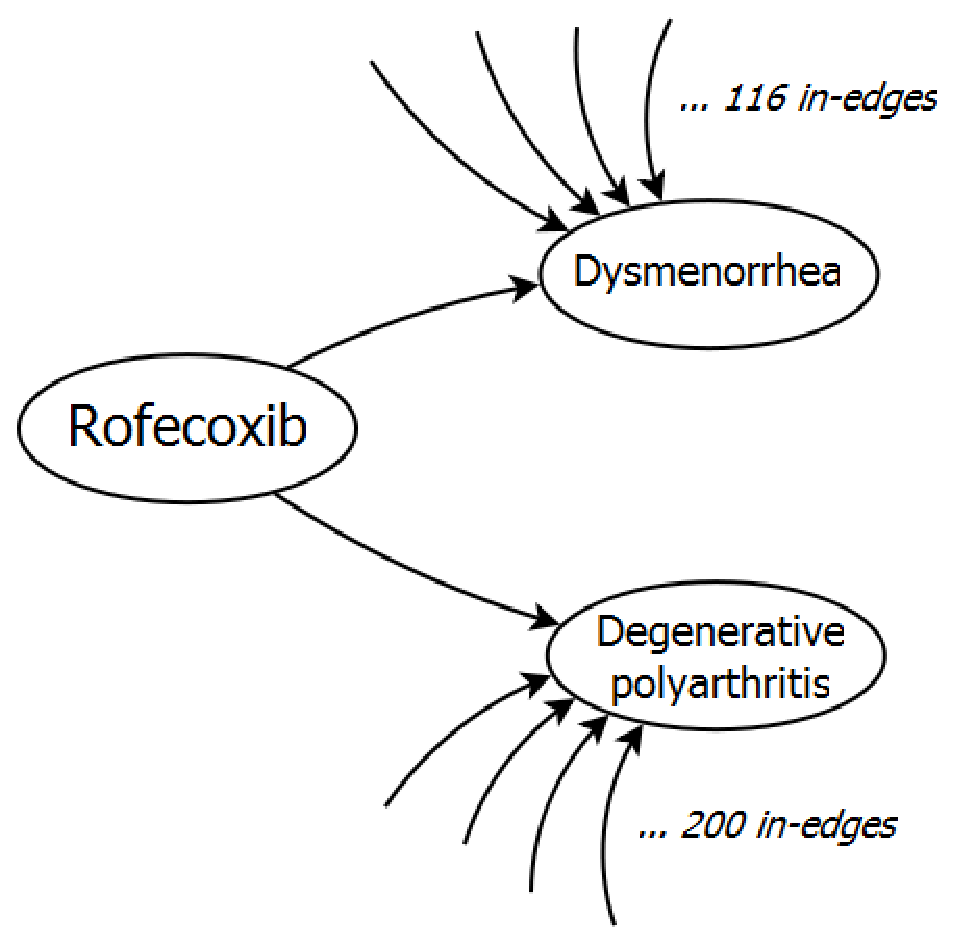
\includegraphics[width=.52\textwidth]{fig/may_treat.eps}
\end{minipage}
\begin{minipage}[c]{0.49\textwidth}\centering
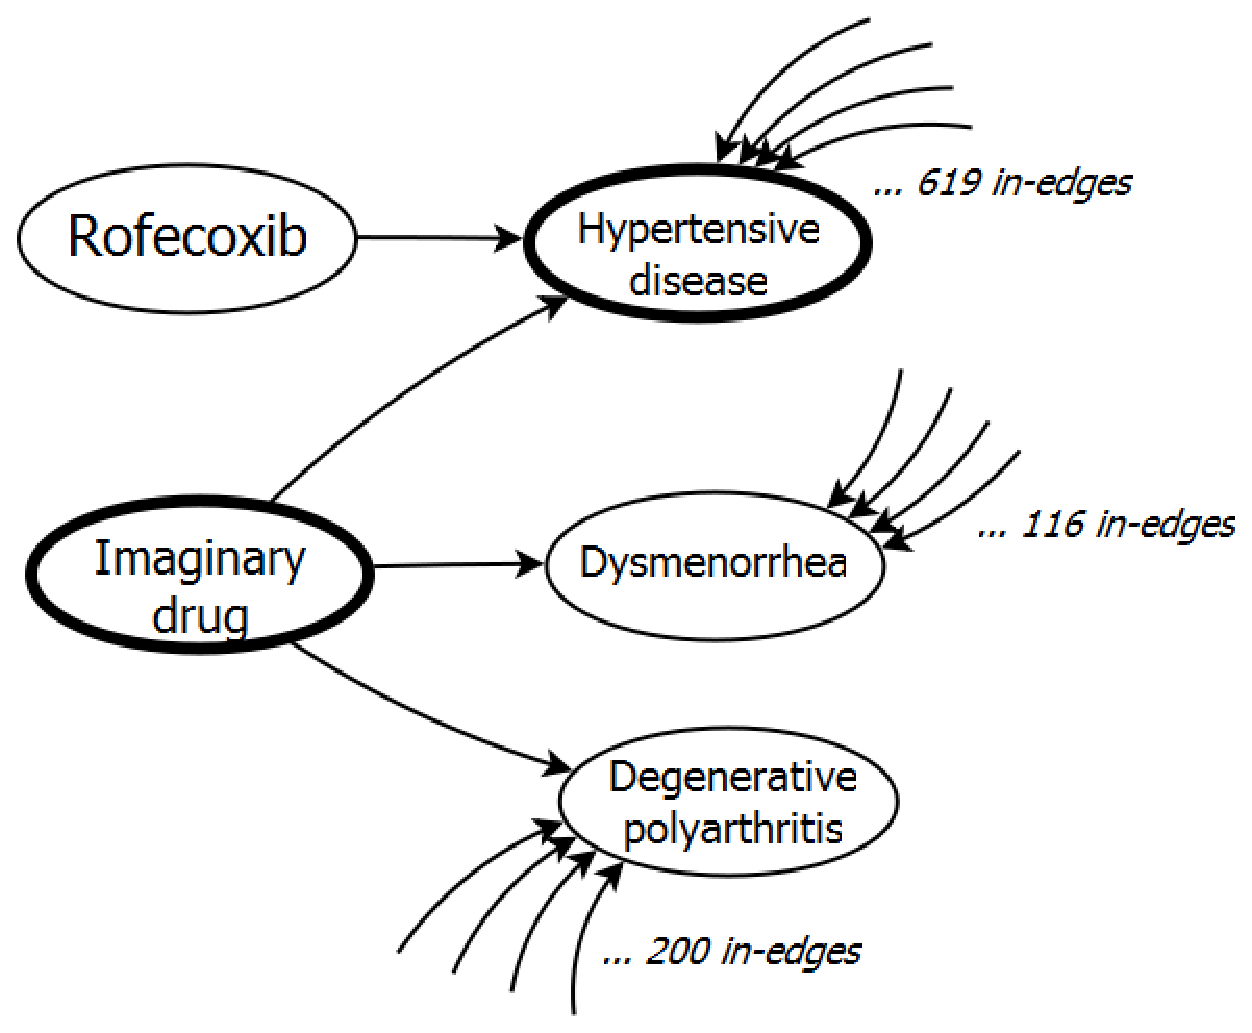
\includegraphics[width=.72\textwidth]{fig/may_treat_augmented.eps}
\end{minipage}
\caption[The may\_treat subgraph]{\label{fig:may_treat} The may\_treat subgraph before and after distortion: The left-hand side of the figure shows the may\_treat subgraph of ground truth relationships between the drug Rofecoxib and two diseases. The right-hand side shows the may\_treat subgraph with some deliberately distorted information.}
\end{figure}

\begin{table*}[tbh]\scriptsize
\begin{center}
\begin{tabular}{ c || c  c || c  c }
\hline
        &   \multicolumn{2}{c||}{w/ noisy may\_treat only}    &   \multicolumn{2}{c}{w/ data and noisy may\_treat}\\
\hline
\hline
       	&   p(\%)   &   rank    &  p(\%)    &    rank    \\
\hline
$\langle Rofecoxib, degenerative~polyarthritis\rangle$       &   3.60e-3   &   555     &   8.14e-3    &   263    \\
$\langle Rofecoxib, dysmenorrhea\rangle$    &   1.54e-2   &   246     &   1.26e-3    &   1703   \\
\hline
\end{tabular}
\end{center}
\caption[Rankings of associations on the noisy may\_treat graph]{\label{tbl:salted_may_treat}Rankings of associations on the noisy may\_treat graph (Figure~\ref{fig:may_treat} right) between Rofecoxib and two diseases derived with and without data.}
\end{table*}

Conversely, we are also interested in learning whether the data graph can help discover patterns in the ontology graph. Figure~\ref{fig:may_treat} (left) shows a subgraph of the NDFRT ``may\_treat" relationship. Rofecoxib is asserted to treat two diseases, namely, dysmenorrhea and degenerative polyarthritis. And there are altogether 116 and 200 drugs that are known to treat dysmenorrhea and degenerative polyarthritis respectively (hence the in-degrees of the nodes). Applying our method on this graph with the query term ``Rofecoxib" yields a similarity-ranked list having degenerative polyarthritis and dysmenorrhea as the top two items. Since this result is the exact ground truth, there is no improvement to be made with the incorporation of the data graph. Therefore, we alter the ground truth graph with some deliberately distorted information, as is shown in Figure~\ref{fig:may_treat} (right), so that the may\_treat graph alone produces only inferior result. More specifically, we specify that Rofecoxib should treat hypertensive disease, the very diseases that is asserted to be treated by the most drugs (a total of 619). Then we add an imaginary drug to treat degenerative polyarthritis, dysmenorrhea, and hypertensive disease. In this way, the original direct connections between Rofecoxb and degenerative polyarthritis and dysmenorrhea become erroneously indirect and are obfuscated by some the noise of high degree nodes along the path. With this scenario, we hope to learn if the incorporation of data graph can correct the misinformation in ontologies.

Table~\ref{tbl:salted_may_treat} shows the result of ranks of the associations between Rofecoxib and degenerative polyarthritis and dysmenorrhea. The ranks of the associations drastically drop to the 555th and 246th respectively on the noisy graph from the top two on the original ground truth graph. This is mainly due to the large node, hypertensive disease, in the middle of the connections. However, with the combined data and may\_treat graph, we notice that the rank of Rofecoxib and degenerative polyarthritis increases to 263rd, while the rank of Rofecoxib and  dysmenorrhea decreases to 1703rd. This shows that the data graph endorses more strongly the association between Rofecoxib and degenerative polyarthritis. Indeed, although Rofecoxib are known to treat both degenerative polyarthritis and dysmenorrhea, the former is a much more popular usage. A search on the National Library of Medicine's PubMed database\footnotemark[1] for ``Rofecoxib and polyarthritis" returns 518 results, while ``Rofecoxib and dysmenorrhea" only returns 29. This result shows that the data graph can help correct misinformation in ontologies to some extent, and in a sense, it also gives a clue of how prior beliefs fit with reality.

\footnotetext[1]{\url{http://www.ncbi.nlm.nih.gov/}}

